\documentclass[12pt]{article}
\usepackage{geometry} 
\geometry{a4paper} 

\usepackage{graphicx}
\usepackage{subcaption}
\usepackage{amsmath}
\usepackage{hyperref}
\usepackage{sectsty}
\usepackage{longtable}
\usepackage{lipsum}
\usepackage{mathpazo}

\allsectionsfont{\normalfont\scshape}

\title{\vspace{-2cm}
\begin{center}
\begin{minipage}{.1\textwidth}

\includegraphics[width=0.8\textwidth]{nyu_seal.png} 
\end{minipage}
\begin{minipage}{.34\textwidth}
\textt{CSCI-UA 473}
\end{minipage}
\end{center}
\vspace{1cm}
\textbf{Random Forests for Music Classification}
\vspace{1cm}}

\author{\textbf{Nicholas Lin}
\\
Department of Computer Science\\
New York University\\
\texttt{nl1637@nyu.edu}}

\date{}

\begin{document}

\maketitle

\begin{center}
    \vspace{1cm}
    \section*{\textbf{Abstract}}
\end{center}

\begin{center}
\end{center}
\vspace{-0.85cm}
I used the features of 50,000 randomly selected songs from a Spotify-released API to investigate the potential of machine learning techniques to classify the genre of songs using only their audio and artistic features. A Random Forest Classifier was given numerical label-encoded genres in order to classify songs based on their features and its performance was then analyzed using One-vs-All ROC curves as well as calculating macro-average AUC score. Model performance was clearly dependent on nature of a musical genre's features and thus suggests that there is merit in potentially exploring further classification attempts for both audio and artistic features in regards to both recommending music to users as well as creating a more diverse music library and architecture.


\newpage

\section{\textbf{Introduction}}
Spotify, the world's leading digital music service, reports over 515 million active listeners, including 210 million premium subscriptions. Its astonishing growth over little more than a decade can be visualized by observing its increases in monthly user growth per quarter as well as yearly revenue growth per year.
\begin{figure}[htbp]
  \centering
  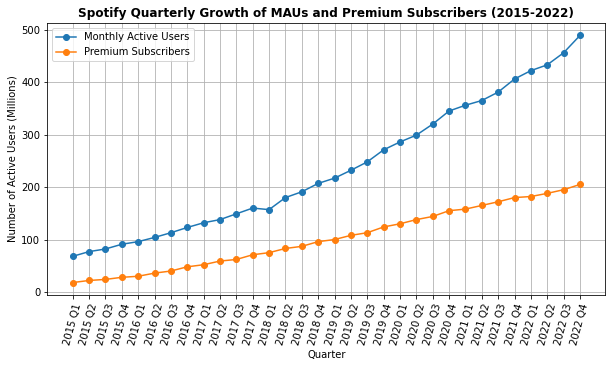
\includegraphics[width=0.7\textwidth]{spotify_growth.png}
  \caption{Spotify Monthly User Growth (2015-2022)}
  \label{Spotify Growth (2015-2022}
\end{figure}

\noindent
Spotify has invested heavily in its recommendation algorithms with over one-third of all new artist discoveries on the platform made through its "Made for You" recommendation sessions. These AI-driven recommendation algorithms are intended to optimize key business metrics such as user retention, time spent on platform, and most importantly generated revenue.

\begin{figure}[htbp]
  \centering
  \vspace{-0.075cm}
  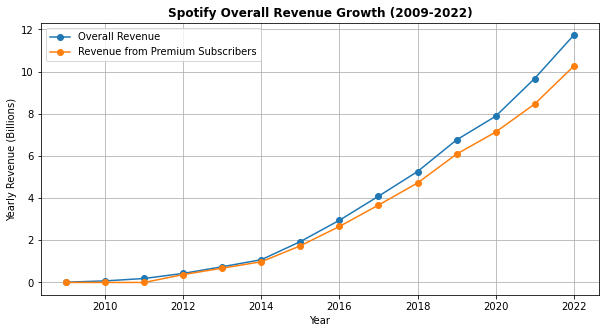
\includegraphics[width=0.7\textwidth]{revenue_growth.png}
  \caption{Spotify Annual Revenue (2009-2022)}
  \label{Spotify Annual Revenue (2009-2022}
\end{figure}

\noindent
And this massive increase in year-to-year generated value can be closely tied to the business' push for more innovative ways to present its media and services for its user base. Several independent machine learning models are used to generate metadata, analyze raw audio signals, utilizing natural language processing (NLP) to analyze lyrics, among other techniques in order to generate user taste profiles as well as to recommend music for users. 
\\ \\
Considering this, I wanted to explore the use of genre-specific audio and artistic feature classifications to determine how effective analysis of a song based only on its audio features and characteristics could be in determining music pertaining to similar categories. By viewing individual songs within Spotify's database solely as a representation of features, I could potentially simplify the process of categorizing music as well as creating simpler relationships between musical characteristics within the feature space.

\section{\textbf{Dataset and Features}}

Spotify reports over 80 million tracks on its platforms and its WebAPI for obtaining a track's audio features was queried by imputation of a track's unique URI or ID. Considering this, I obtained a dataset of 50,000 random Spotify tracks originating from this API which were distributed between 10 unique genres: Electronic, Anime, Jazz, Alternative, Country, Rap, Blues, Rock, Classical, and Hip-Hop. 
\\ \\
While there were 10 unique genres, there were 18 features for each queried track. From these 18 features, I immediately dropped \textit{artist\_name}, \textit{instance\_id}, \textit{track\_name}, and \textit{obtained\_date}. The remaining features are shown below with their feature name, data type, and a short description

\begin{longtable}{|l|c|p{6cm}|}
\hline
\textbf{Feature Name} & \textbf{Data Type} & \textbf{Description} \\
\hline
\endfirsthead
\multicolumn{3}{c}%
{\tablename\ \thetable\ -- \textit{Continued from previous page}} \\
\hline
\textbf{Feature Name} & \textbf{Data Type} & \textbf{Description} \\
\hline
\endhead
\hline
\multicolumn{3}{r}{\textit{Continued on next page}} \\
\endfoot
\hline
\endlastfoot
popularity & float64 & Measure of popularity of track   
(0.0 - 100.0) \\
\hline
acousticness & float64 & Confidence measure of whether track is acoustic (0.0 - 1.0) \\
\hline
danceability & float64 & How suitable track is for dancing based on a combination of musical elements (0.0 - 1.0) \\
\hline
duration\_ms & float64 & Track duration (ms)\\
\hline
energy & float64 & Perceptual measure of intensity and activity (0.0 - 1.0) \\
\hline
instrumentalness & float64 & Prediction of whether track contains vocals (0.0 - 1.0) \\
\hline
key & object & Key which the track is in (-1 - 11) \\
\hline
liveness & float64 & Detects presence of audience in recording (0 - 1.0) \\
\hline
loudness & float64 & Overall loudness of a track measured in decibels (-60 - 0) \\
\hline
mode & object & Indicates track modality (0 or 1) \\
\hline
speechiness & float64 & Detects presence of spoken words in track (0 - 1.0) \\
\hline
tempo & object & Overall estimated tempo in beats per minute (BPM) \\
\hline
valence & float64 & Describes musical positiveness conveyed by track (0 - 1.0) \\
\hline
\caption{Spotify Dataset Audio Features}
\end{longtable}


\section{\textbf{Pre-Classification Methods}}
Before training the classification model, I pre-processed the dataset, being sure to remove both missing values as well as standardize feature data types. I split the data into a 80/20 training/test splits before dimensionality reducing the data. After this I ran a clustering algorithm on the data.
\subsection*{\textbf{Preprocessing}}
After summing all missing values within the data, I determined there were only 5 songs which were missing all of their features. I removed these songs before type-converting certain features like \textit{valence} and \textit{tempo}, which were numerical values that weren't being represented as floats. \\ 

\noindent
Converting categorical labels and data into numeric representations was next, such as mapping \textit{key} to numbers for example mapping "C" to 0 or "G\#" to 7. \textit{mode} was then dummy-coded, creating two new features "mode\_Major" and "mode\_Minor". Finally I mapped \textit{genre}, the target variable, to numerical labels. \\

\noindent
For training/test split of the dataset, given 5,000 songs for each genre, I randomly selected 500 songs from each genre to be used within the test set while the remaining 4,500 songs were used within the training dataset.

\section*{\textbf{Dimensionality Reduction}}
Given the feature complexity and how high-dimensional the dataset was, dimensionality reduction before any classification step was undertaken was crucial as it would improve model training time and performance, correct any multi-collinearity, as well as help to visualize the dataset in varying dimensions.

\subsection*{\textbf{Principal Component Analysis (PCA)}}
Multi-collinearity was a concern as song features could have been correlated, for example songs with higher energy would generally have higher tempo. Running PCA on this data before classification could result in the first few principal components explaining a large portion if not a majority of the data variance. \\ \\
Analyzing the Scree Plot allows for understanding of individual feature contribution to variance of the data 

\begin{figure}[htbp]
  \centering
  \vspace{-0.075cm}
  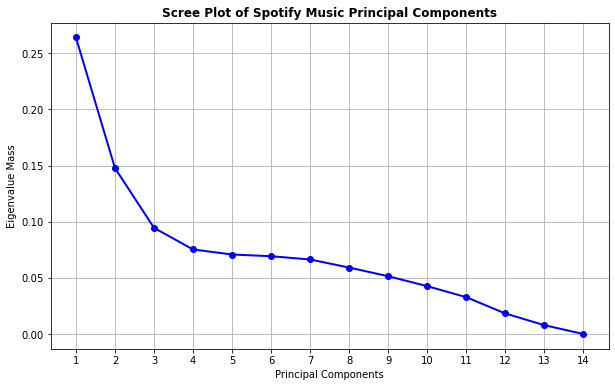
\includegraphics[width=0.65\textwidth]{pca_scree.png}
  \caption{Scree Plot of Feature Explained Variance)}
  \label{PCA Scree Plot}
\end{figure}

\noindent
It was necessary to decide the optimal number of components to use for the PCA, which I decided to set as features with eigenvalue masses above \textbf{0.05}. In doing so, I was left to train a PCA with 9 principal components and fit it onto both the training and test data. Now having the PCA-reduced dataset, I wanted to visualize each principal component

\begin{figure}[htbp]
  \centering
  \vspace{-0.075cm}
  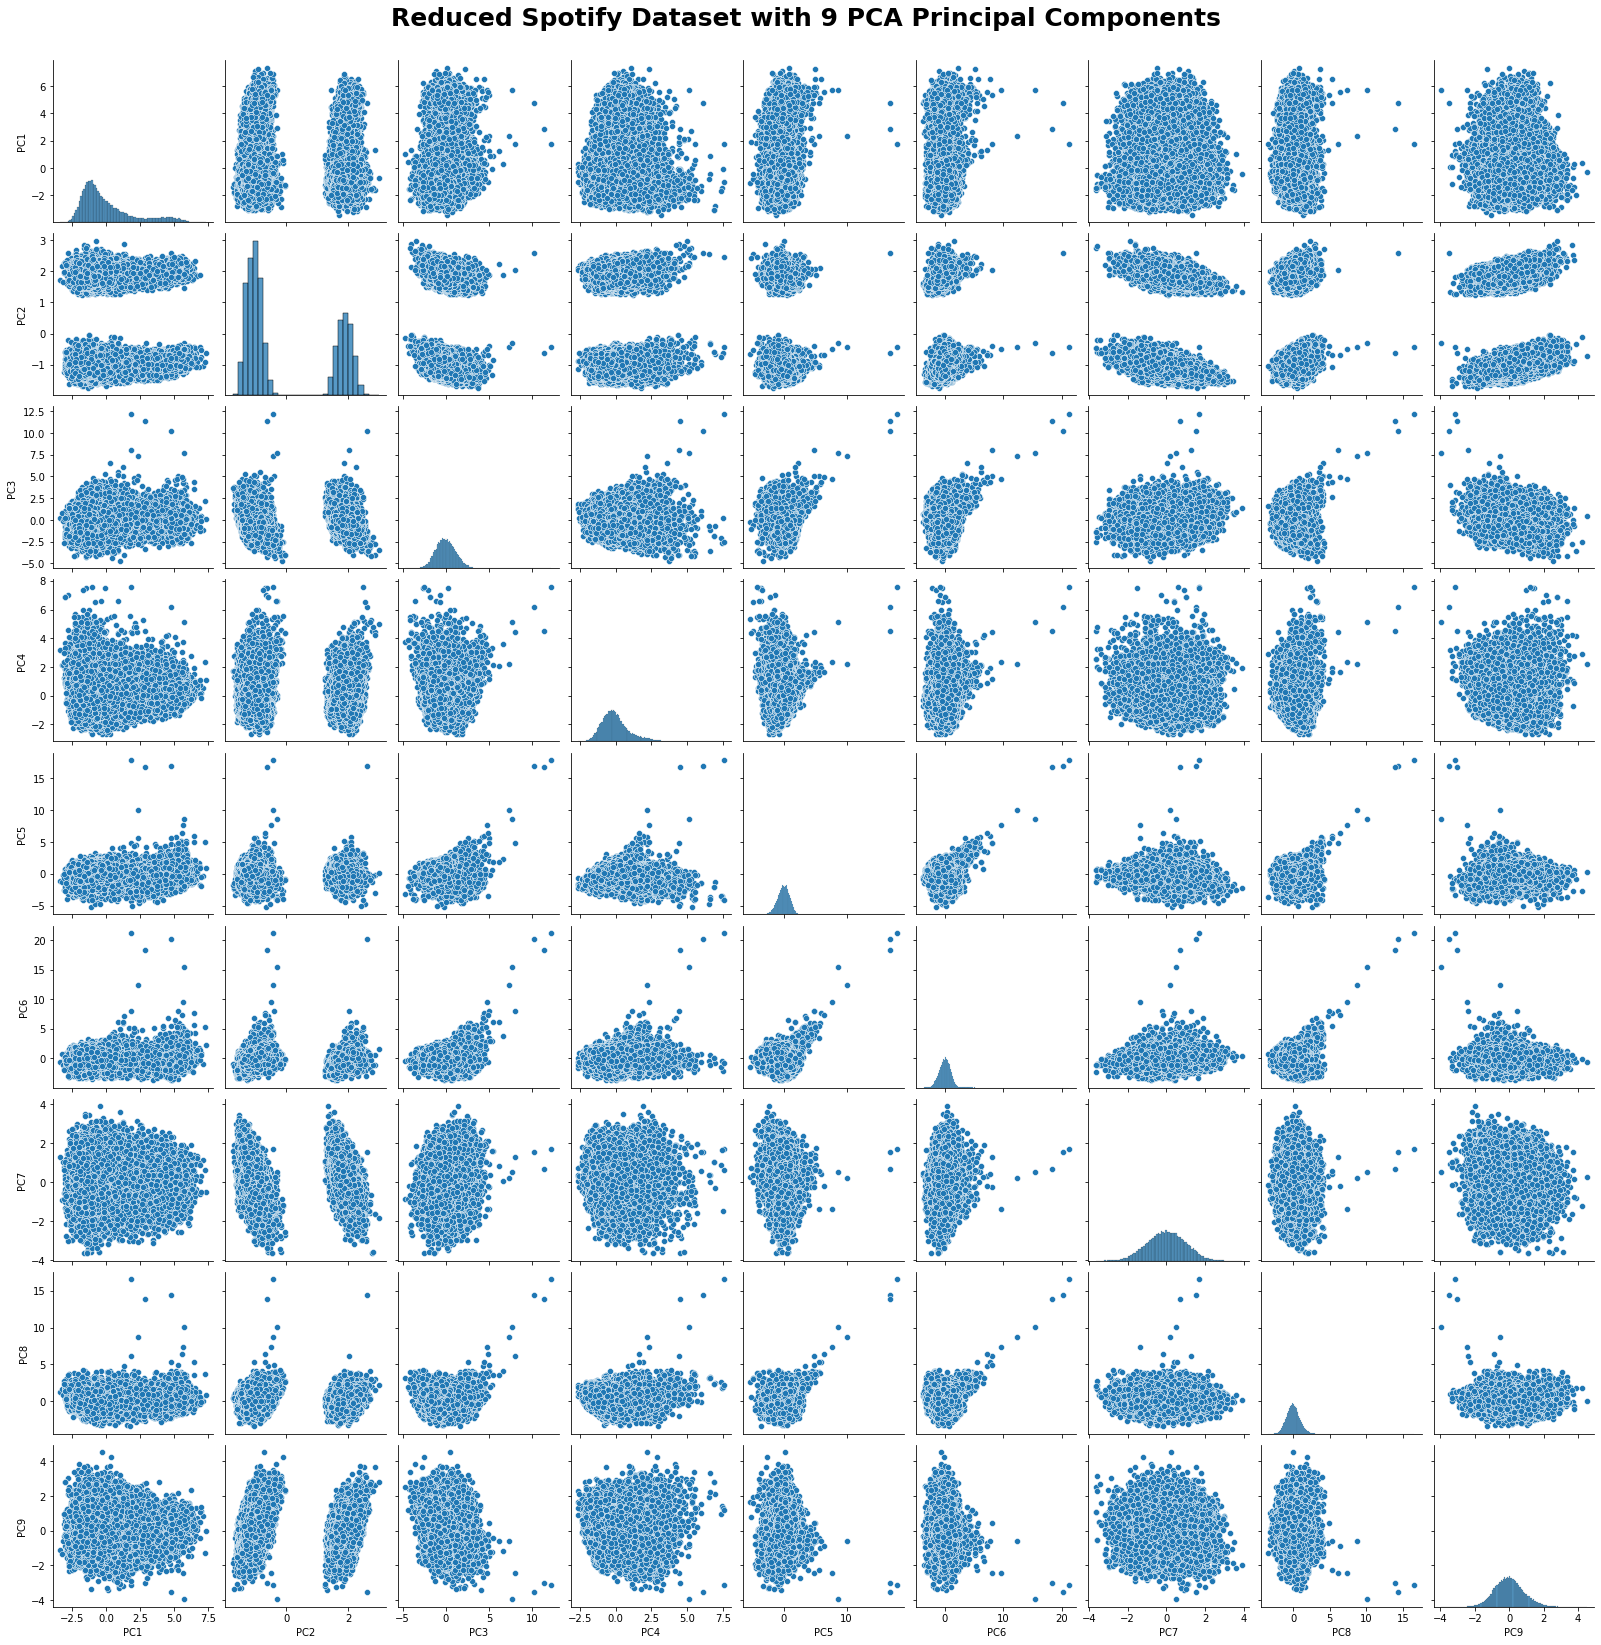
\includegraphics[width=0.6\textwidth]{9_pca.png}
  \caption{PCA Reduced Spotify Dataset}
  \label{PCA Scree Plot}
\end{figure}

\noindent
Looking at both the Scree Plot and the PCA-reduced dataset, the first principal component contains the most eigenvalue mass with the other features dropping off quite significantly. The decision to include 9 principal components decently explains the majority of data variance while reducing the complexity of both the data and the eventual model training process.

\section*{\textbf{Clustering}}
KMeans clustering was implemented as it would allow for the grouping of songs with similar features to create an underlying structure within the data to enhance the subsequent training of a Random Forest Classifier.

\subsection*{\textbf{Optimal Clusters for KMeans}}
KMeans clustering segregates the PCA-reduced dataset into \textit{k} clusters. However determination of optimal number of clusters to train was crucial thus I used two methods to make this distinction, the \textbf{silhouette scores} of a range of clusters and the \textbf{within-cluster sum of squares (WCSS)} metric for the elbow criterion. I first analyzed the silhouette scores of a range of clusters


\begin{figure}[htbp]
  \centering
  \vspace{-0.075cm}
  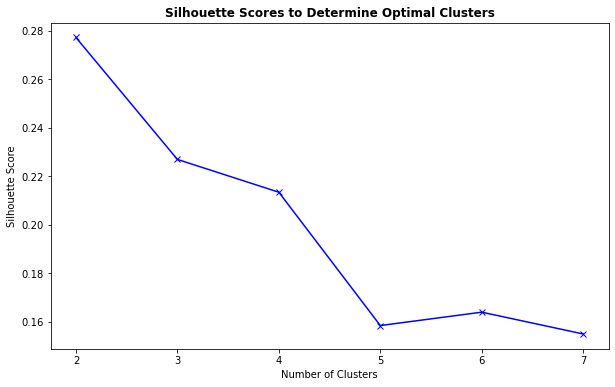
\includegraphics[width=0.65\textwidth]{kmeans_silhouette.png}
  \caption{Silhouette Score of KMeans Clusters}
  \label{KMeans Silhouette Scores}
\end{figure}


\noindent
The silhouette score measures how similar a sample is within its own cluster compared to other clusters. Analyzing the silhouette scores here, it is noticeable that the steepest drop-off of silhouette scores is at the \textbf{fourth} cluster. We want to aim for the the number of clusters in which the silhouette score is the highest, which leaves us with a choice of either 2 clusters, which gives the highest silhouette score, or 4 clusters after which the silhouette score drops off rapidly. \\ 

\noindent
Given these choices, I still needed to consider the elbow criterion to determine a final number of clusters to train for my KMeans model. For the elbow method, the sum of squared distances is calculated from each point to its assigned center and a within-cluster sum of squares (WCSS) score is calculated to determine which number of cluster results in the lowest WCSS score for the  model


\begin{figure}[htbp]
  \centering
  \vspace{-0.075cm}
  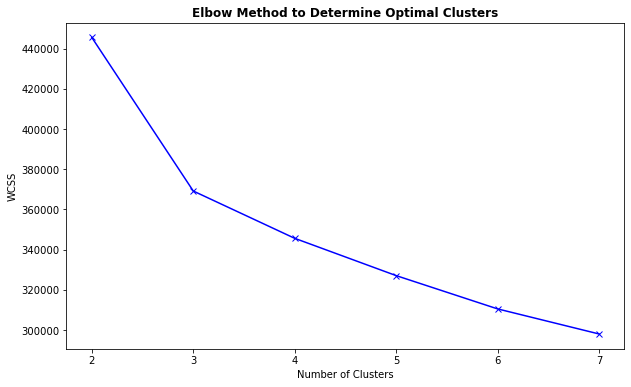
\includegraphics[width=0.65\textwidth]{kmeans_elbow.png}
  \caption{Within-Cluster Sum of Squares}
  \label{KMeans Elbow Criterion WCSS}
\end{figure}

\newpage \noindent
Its clear that the WCSS decreases as the number of clusters increases. However given the previous choices of clusters for their respective silhouette scores, it should be noted that the decrease in WCSS from 2 clusters to 3 is incredibly steep and continues to decrease for 4 clusters. Given this, a conclusion can be made that the optimal number of clusters to train a KMeans model on is 4.


\subsection*{\textbf{KMeans Clustering}}
I moved to fit the KMeans model onto the dataset. Using 4 clusters, I first trained the model before fitting it to the PCA-transformed data. This allowed me to create a new feature within the original dataset based on the class which the KMeans model fit the data to. This new feature would be the label for the cluster within the original. \\

\noindent
Displaying the actual clusters within the dataset allowed for both visualization of data points through the data as well as each assigned cluster label

\begin{figure}[htbp]
  \centering
  \vspace{-0.075cm}
  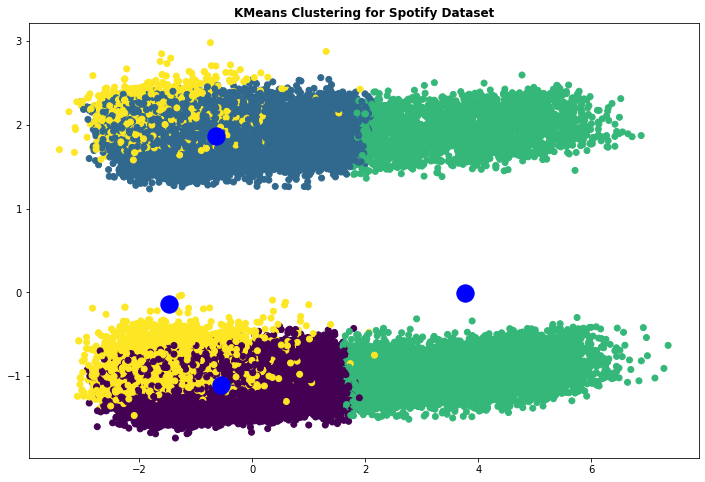
\includegraphics[width=0.9\textwidth]{kmeans_clustering.png}
  \caption{Spotify KMeans Labels with 4 Clusters}
  \label{Spotify KMeans labeling}
\end{figure}

\section{Random Forest Classification}
Random Forests are incredibly robust in handling higher-dimensional datasets when compared to other classification models. Additionally its propensity for capturing non-linear relationships between feature and target variables, combined with the fitting of PCA and KMeans beforehand, would expose further relationships between both songs and genre classification. 

\subsection*{Cross-Validation for Hyperparameter Optimization}
Hyperparameter tuning allows for control of model complexity which greatly impacts bias-variance tradeoff. Additionally although Random Forests innately don't tend to overfit when training, hyperparameter optimization allows for the model to generalize more effectively to new data. \\

\noindent
I did this by training multiple Random Forest models over a variety of hyperparameters such as \textbf{number of trees}, \textbf{maximum depth}, \textbf{minimum samples required to split a node}, \textbf{minimum samples per leaf}, and \textbf{whether or not sample is bootstrapped}. \\ 

\noindent
Using cross-validation, the optimal hyperparameters were a forest with 500 trees, max depth of 10, min samples of 4 samples per leaf node, min 10 samples to split a node, and having sub-sample size controlled for.

\subsection*{Training the Random Forest}
Given the optimal hyperparameters, I trained the Random Forest Classifier and then fit it to the data. From this I used the model to predict the target variable using the cluster-labeled dataset. Comparing the predicted target variable with the actual test dataset target variable resulted in a classification report of the precision, recall, and F1 score of the classifier \\

\begin{figure}[h]
    \centering
    \begin{subfigure}{0.45\textwidth}
        \centering
        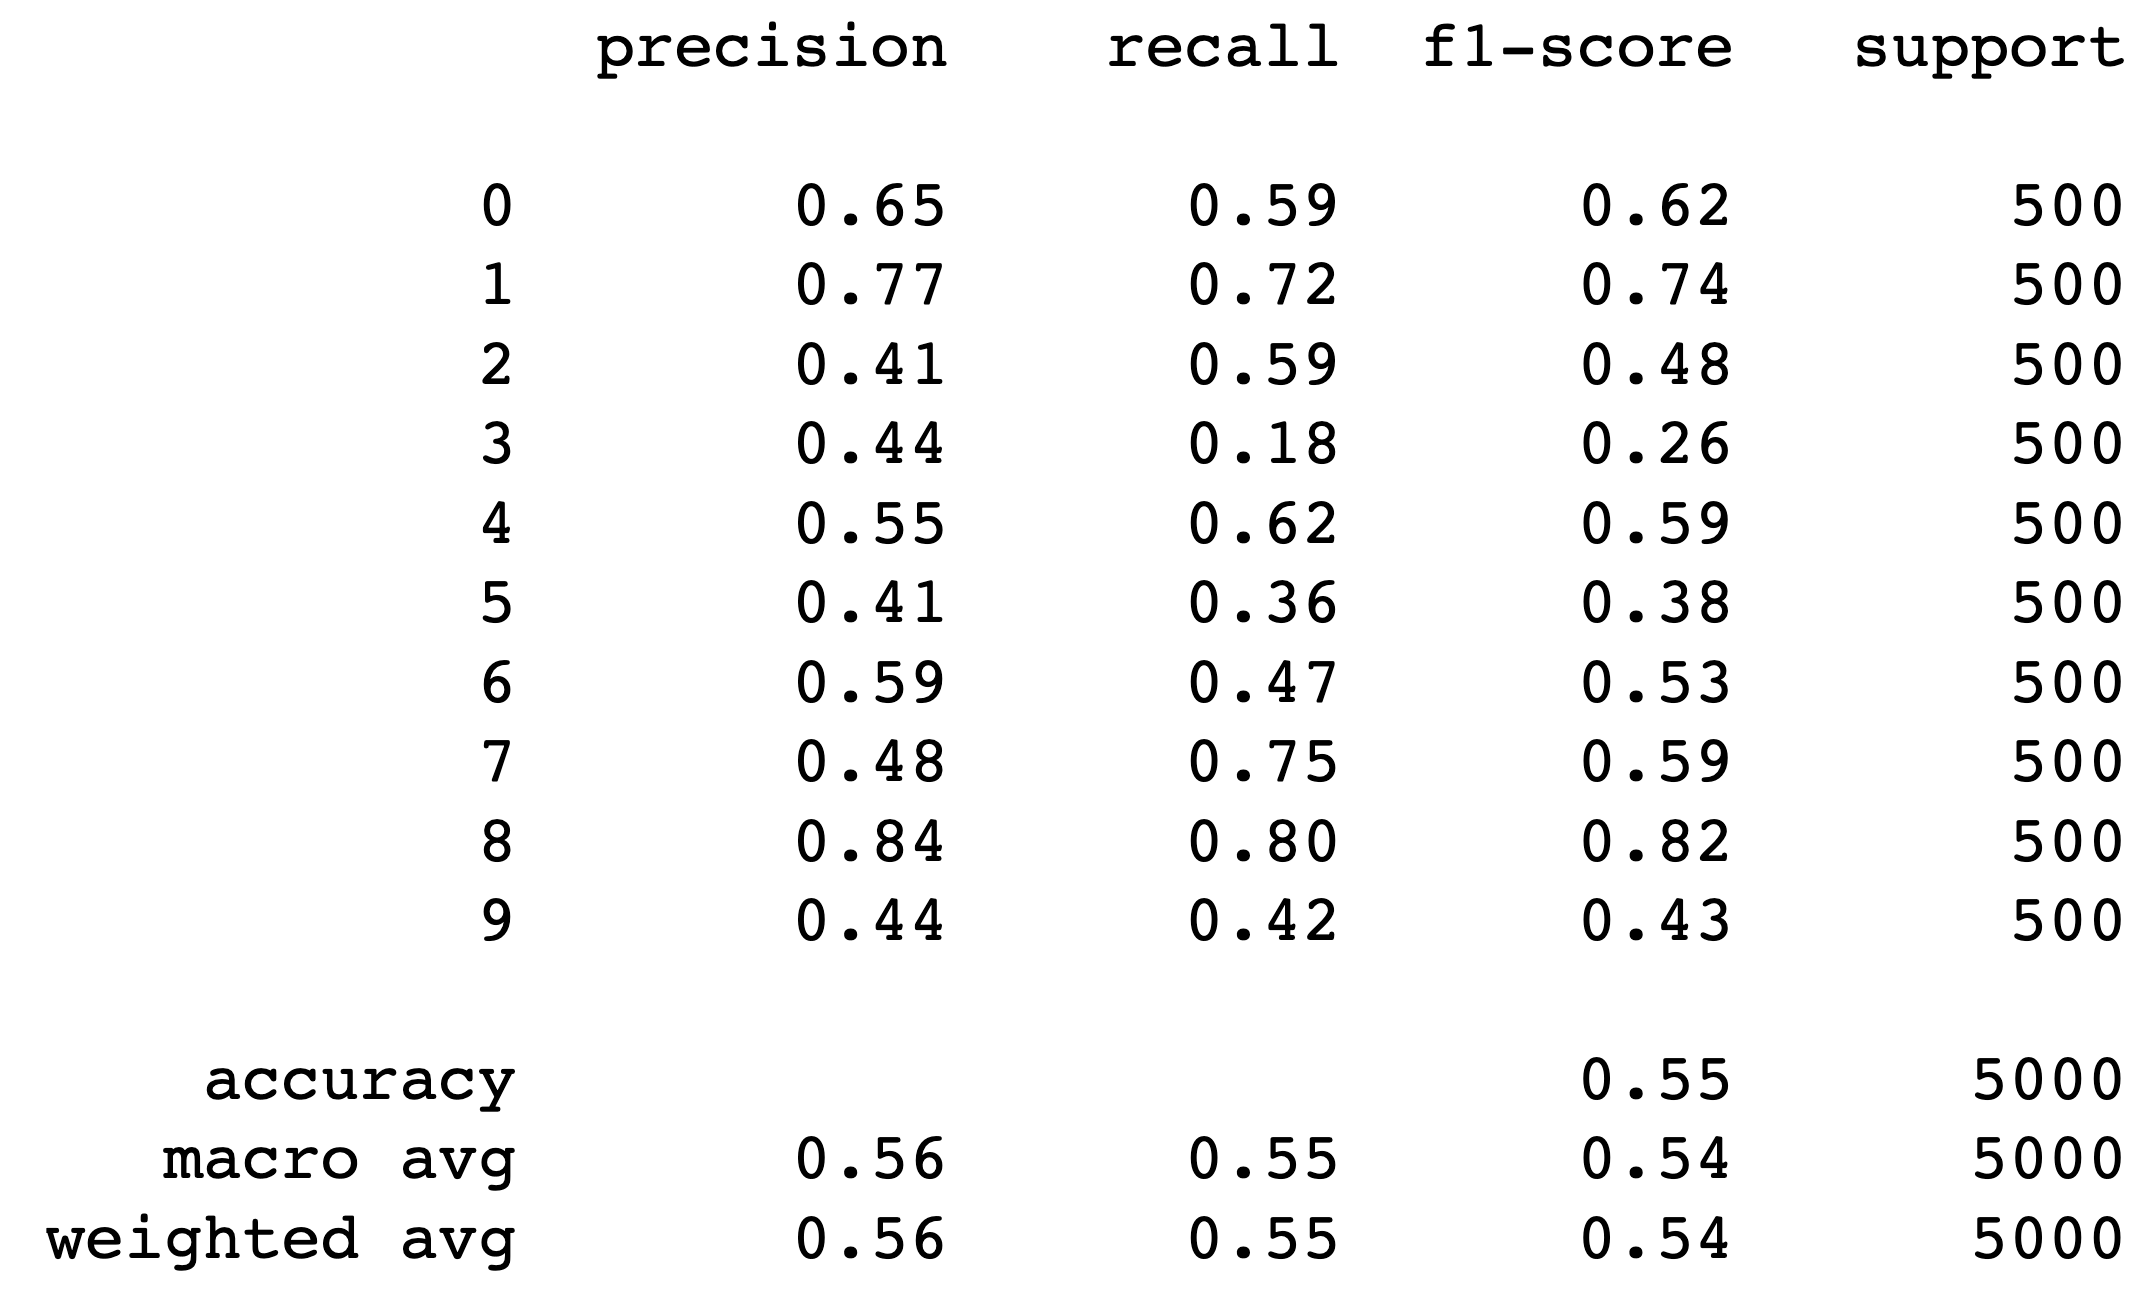
\includegraphics[width=\textwidth]{classification_report.png}
        \caption{Random Forest Classification Report}
        \label{fig:image1}
    \end{subfigure}
    \hfill
    \begin{subfigure}{0.45\textwidth}
        \centering
        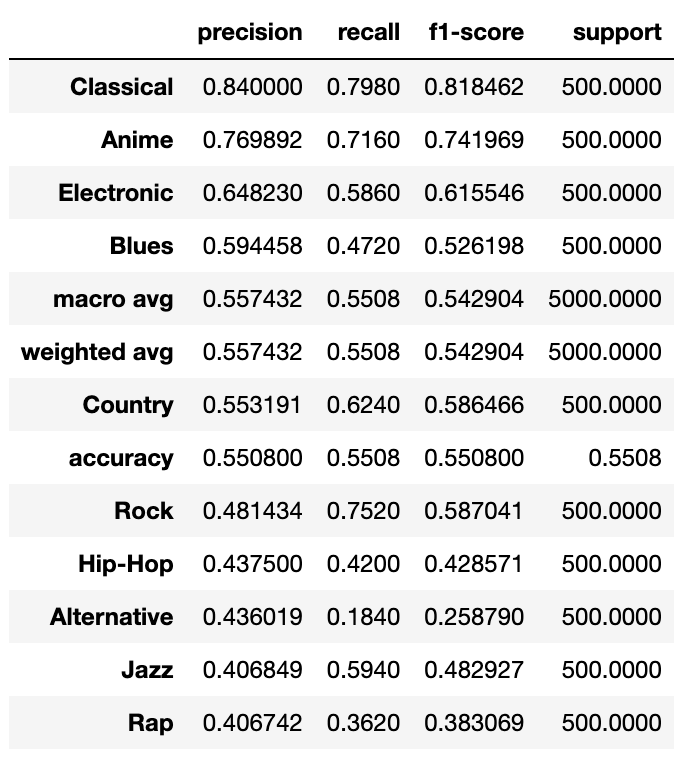
\includegraphics[width=\textwidth]{classification_df.png}
        \caption{Random Forest DataFrame}
        \label{fig:image2}
    \end{subfigure}
    \caption{Random Forest Classification Values}
    \label{fig:double_image}
\end{figure}

\noindent
However without categorical labels, the genre numerical labels didn't reveal much about the data. Because of this, I converted the classification report into a Pandas DataFrame, inverted the original genre mapping so it became the index of the DataFrame, and then sorted this new DataFrame by precision values. Both the initial Random Forest classification report as well as the Random Forest classification DataFrame are displayed

\newpage
\section{Classifier Evaluation}
As can clearly be seen, the model obtained the best performance in terms of classifying \textbf{Classical} and \textbf{Anime} music, while having the worst performance on classifying \textbf{Rap} and \textbf{Jazz} music in terms of precision, recall, and F1 score. However this wasn't enough to evaluate the model on. 

\subsection*{Multi-Class Classification Evaluation}
In most cases a ROC curve and AUC metrics would be simply enough to evaluate a binary classification model. However I was working with multi-class classification in this context so there were essentially two approaches I could've taken to determine model performance. The first was one-vs-all in which a single classifier is trained for each class and it labels samples of that class as positive while it labels the rest as negative. The other option was one-vs-on in which a separate model is trained for every pair of classes. \\

\noindent
I decided to implement one-vs-all given that the classification of each genre was being tested against its similarities to other genres on the same features. Within this ROC curves were calculated for each individual one-vs-all classification model as well as the AUC for each model displayed \\


\begin{figure}[htbp]
  \centering
  \vspace{-0.075cm}
  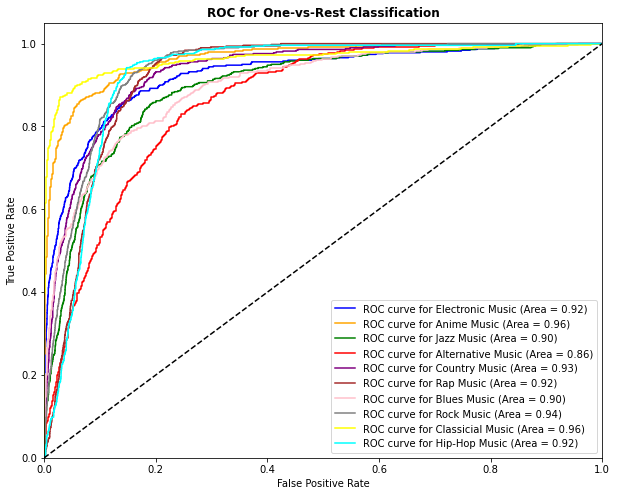
\includegraphics[width=0.8\textwidth]{one-vs-all.png}
  \caption{One-vs-All ROC Curves and AUC by Genre}
  \label{One-Vs-All Graph}
\end{figure}

\noindent
Along with this, the macro-average AUC score of the One-vs-Rest classification models was \textbf{0.7504}. It can be seen that although in terms of precision and recall for the original model being low for genres such as \textbf{Rap} and \textbf{Jazz}, the one-vs-all ROC curves are actually quite promising as well as having a relatively high AUC score for all genres. 

\section{Discussion}
As previously discussed, the ROC curves and the AUC for each individual genre within One-vs-All classification was incredibly high with the highest AUC being \textbf{0.96} and the lowest AUC being just \textbf{0.86}. Even the macro-averaged AUC score being \textbf{0.7504} wasn't that poor for such a dataset. \\

\noindent
It is important to address here the motivations behind why the classification was so successful for some genres while still requiring further optimization for other genres. Features like \textit{acousticness}, \textit{danceability}, \textit{speechiness}, and even \textit{mode} created essentially a comprehensive and diverse description of every song but skewed towards certain genres. The model performed best on genres such as \textbf{Classical}, \textbf{Anime}, and \textbf{Electronic} likely because these genres do not depend on how lyrical the music is as much as the underlying musical score. In the same vein, the model performing worst on genres such as \textbf{Rap} and \textbf{Jazz} happen to coincide with these genres being characterized by the contents and meanings of the lyrics rather than the accompanying musical score.

\section{Future Work}
It is interesting to be able to visualize the impact of classification models on interpreting musical style and genres from just the features of a particular song. In this case I had built a Random Forest model which had quite accurately been able to classify the songs within the Spotify dataset. Even more importantly however was that the Random Forest had essentially classified the music genres in a tangible way. It classified the music in a way that made logical sense, with certain features leaning heavily towards some genres of music while other genres of music emphasized other features. \\

\noindent
In this way it is interesting to discuss the efficacy of machine learning algorithms, and in particular classification models, to address the business needs of a company like Spotify which values data insights into their users and business. Understanding the power of presenting music to its users has been what has underlied Spotify's meteoric rise to become an industry leader. Its presentation of songs within its "Made for You" recommendation service has become a huge draw within its userbase, and understanding which aspects of songs make them unique as well as which aspects allow them to fit a certain niche is the foundhttps://www.overleaf.com/project/646d8e2b74d7f1faa7f20ffeation of these algorithms. \\

\noindent
Therefore given that model performance clearly was dependent on the nature of a musical genre's inherent features, this suggests that there is merit in potentially exploring further classification attempts for both audio and artistic features, in particular in regards to recommending new music to users as well as providing a more diverse music library and architecture.


\end{document}